% ============================================================
% Faster-GS: Morton Z-order reordering
% ============================================================

\begin{frame}{Morton Z-order reordering --- tăng locality bộ nhớ}
\footnotesize
\begin{itemize}
    \item \textbf{Bước 1 --- Lượng tử hoá:} toạ độ mỗi Gaussian được đưa về 10 bit/trục trong bounding box của toàn bộ point cloud.
    \item \textbf{Bước 2 --- Spread bits (part1by2):} giãn mỗi số 10-bit thành 30-bit bằng magic-number bit trick, rồi ghép 3 trục:
    \[
        M = \text{spread}(q_x) \;\mathrel{\mathrm{OR}}\; \big(\text{spread}(q_y)\ll 1\big) \;\mathrel{\mathrm{OR}}\; \big(\text{spread}(q_z)\ll 2\big)
    \]
    \item \textbf{Bước 3 --- Sắp xếp:} toàn bộ Gaussian được \texttt{argsort} theo $M$ tăng dần --- đây chính là thứ tự duyệt theo \textbf{đường cong Z-order}: 2 điểm gần nhau trong không gian 3D thường có mã Morton gần nhau.
    \item[$\Rightarrow$] Gaussian trong cùng 1 tile màn hình thường gần nhau trong bộ nhớ sau reorder $\Rightarrow$ cache GPU hit rate cao hơn khi rasterizer tile-based duyệt danh sách Gaussian mỗi tile.
    \item Luôn chạy mỗi \texttt{morton\_reorder\_interval=5000} iteration (trước đây mặc định \texttt{0}, tức tắt hẳn).
\end{itemize}
\centering
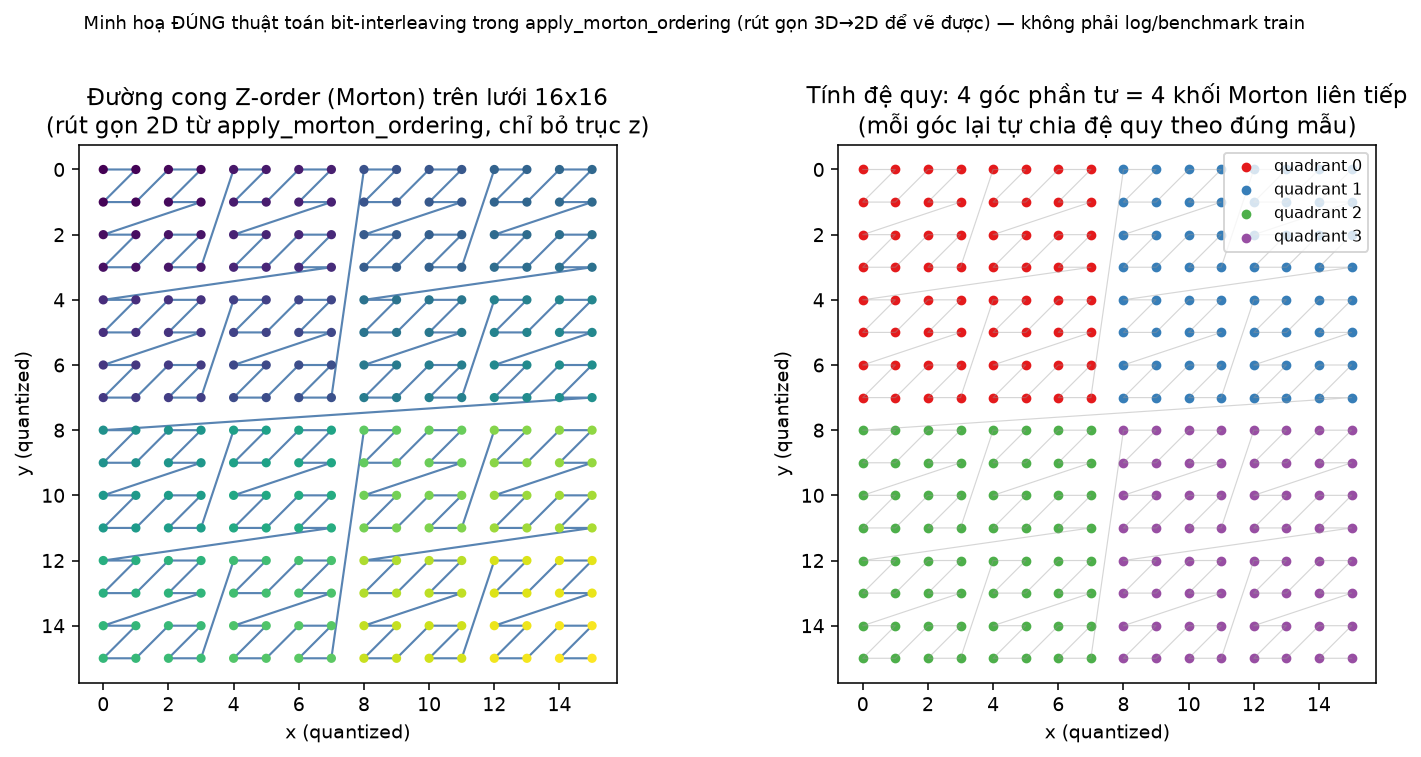
\includegraphics[width=0.38\linewidth]{../BOOK/fastergs_merge_figures/09_morton_zorder_curve.png}
\captionof{figure}{\footnotesize Đường cong Z-order thật (chạy đúng thuật toán spread-bits, rút gọn 3D$\to$2D để vẽ)}
\end{frame}
